\documentclass[a4paper,11pt,twoside]{article}
%\documentclass[a4paper,11pt,twoside,se]{article}

\usepackage{UmUStudentReport}
\usepackage{verbatim}   % Multi-line comments using \begin{comment}
\usepackage{courier}    % Nicer fonts are used. (not necessary)
\usepackage{pslatex}    % Also nicer fonts. (not necessary)
\usepackage[pdftex]{graphicx}   % allows including pdf figures
\usepackage{listings}
\usepackage{pgf-umlcd}
%\usepackage{lmodern}   % Optional fonts. (not necessary)
%\usepackage{tabularx}
%\usepackage{microtype} % Provides some typographic improvements over default settings
%\usepackage{placeins}  % For aligning images with \FloatBarrier
%\usepackage{booktabs}  % For nice-looking tables
%\usepackage{titlesec}  % More granular control of sections.

% DOCUMENT INFO
% =============
\department{Department of Computing Science}
\coursename{Object-Oriented Programming Methodology 7.5 p}
\coursecode{5DV133}
\title{OU4 Sensor Network}
\author{Johan Eklund ({\tt{kv03jed@cs.umu.se}}) \\ 
Tommie Lindberg ({\tt{c15tlg@cs.umu.se}}) \\
Jakob Lundin ({\tt{c14jln@cs.umu.se}}) \\
Lorenz Gerber ({\tt{dv15lgr@cs.umu.se}}, {\tt{lozger03@student.umu.se}})
}
\date{2016-05-23}
%\revisiondate{2016-01-18}
\instructor{Anders Broberg \\ Niklas Fries \\ Adam Dahlgren \\
  Jonathan Westin \\ Erik Moström \\ Alexander Sutherland}


% DOCUMENT SETTINGS
% =================
\bibliographystyle{plain}
%\bibliographystyle{ieee}
\pagestyle{fancy}
\raggedbottom
\setcounter{secnumdepth}{2}
\setcounter{tocdepth}{2}
%\graphicspath{{images/}}   %Path for images

\usepackage{float}
\floatstyle{ruled}
\newfloat{listing}{thp}{lop}
\floatname{listing}{Listing}



% DEFINES
% =======
%\newcommand{\mycommand}{<latex code>}

% DOCUMENT
% ========
\begin{document}
\lstset{language=C}
\maketitle
\thispagestyle{empty}
\newpage
\tableofcontents
\thispagestyle{empty}
\newpage

\clearpage
\pagenumbering{arabic}

\section{Introduction}
In predefined groups of students we were asked to create a simulation
of a network consisting of a number of \textit{nodes} with a short
communication range \cite{sensornetwork}. The simulation consits of
time steps, for every time step the network goes through the network
and node and makes sure it does its job.

Using the \textit{rumour routing} algorithm \cite{braginsky2002} you
start with a network of \textit{nodes}, in the  network there are
\textit{messages}, signals, that travel the network to
collect and to share information. These messages have a set amount of
steps they can make before they vanish. The nodes detect unique
\textit{events} and \textit{queries} can be made in any node for that
event, the network will then send the \textit{query} to find the
\textit{node} that detected the \textit{event}.

Communication is done by using the rumour-routing algorithm
\cite{braginsky2002}. An event in the simulation is an ID, a time
stamp and a  position of where it happened. Nodes knows its neighbors
and they are static in the grid. Nodes can have a maximum of 8
neighbors depending on location. Nodes have have a table of events and
know how far away every other node is. Nodes generate messages in the
form of agents and queries. Queries should come back to the node
within 45 steps if not the node should send another one. Queries are
messages that carries the information of an event it's trying to find
and a stack of nodes it has traveled through. The node the query
passes through checks it's table to see if it know about the event, if
it finds it it will send the query on its way to the event node. If it
doesn't find it, it will send it to a random neighbor. If a query
finds its target node it will get sent back to its original node the
same way it got to the event so it can report about it.

In our simulation a query will vanish if it can't find the event in 45
steps. Agents are messages that carry a table of events and the path
to these events. The agents travel through the network and
synchronizes with the nodes it passes. The events with the shortest
distance gets saved in both the nodes and the agents tables. In our
simulation the agents will vanish in 50 steps. In our simulation
agents have a 50\% chance to be generated when an event is
detected. In our simulation the network is 50 by 50 and runs for
10000 time steps. Every 400 time steps four randomly chosen nodes are
supposed to generate queries.

\section{Compiling and Running of the Program}

The program is written according to Java 1.7 and compiles on the
commandline with standard command \texttt{javac RumourRoutingApp.java}.
Invoking the compiled program is done by calling \texttt{java
  ./RumourRoutingApp.class} from the command line.
A typical run will result in screen output similar to the following:
\begin{verbatim}
Event at x: 30 y 120, at time 1135, id 317
Event at x: 210 y 20, at time 1040, id 286
Event at x: 0 y 50, at time 1422, id 389
Event at x: 150 y 250, at time 1410, id 385
Event at x: 130 y 0, at time 1826, id 490
Event at x: 130 y 220, at time 3002, id 748
Event at x: 50 y 270, at time 4546, id 1164
Event at x: 130 y 210, at time 3848, id 977
Experiment finished
\end{verbatim}

A number of parameters can be modified in the
\texttt{RumourRoutingApp.java} file. The meaning of these will be
described in the section `Description of Program Structure'.
\begin{verbatim}
int NODES_X                 = 50;
int NODES_Y                 = 50;
int NO_NODES                = NODES_X * NODES_Y;
double NEW_EVENTS           = 0.0001;
int NODE_RANGE              = 15;
double PROB_AGENT           = 0.5;
int TTL_AGENT               = 10;
int TTL_QUERY               = 50;
int QUERY_NODES             = 4;
int QUERY_PERIODICITY       = 400;
int TIMESTEPS               = 10000;
int NUMBER_OF_RECENT_NODES  = 5;
int QUERY_RESEND_WAIT       = TTL_QUERY *8;
\end{verbatim}



\subsection{Javadoc}
JavaDoc pages were created with the built-int functions in IntelliJ
and can be found in the javadoc subdirectory. The pages are in HTML
format and can be viewed by opening index.html in the javadoc
directory with a web browser.



\section{General Program Structure}
The design of our rumour routing implementation from `OU3' assignment
proofed to be mostly feasible for implementation. Certainly, some
details that were left open in the design slightly changed other
structures, but mostly the presented code can be seen as
an implementation of `OU3'. Hence below follows just a rather short
account for the general design and we will focus more on practical
implementation details.

A general aim of object oriented design is to develop a model where
real world entities have their counterparts modelled as classes/objects
with similar properties, behaviour and relations. For the current
implementation, the real world entities of interest are sensor
\textit{nodes} with the capability to detect events and send/receive
information. These three activities define two other abstract real
world entities: \textit{events} and \textit{messages}. The former are
\textit{detected} and the latter can be \textit{sent} and \textit{received}. 
Finally, as we are interested to investigate specific
situations involving a large number of the above mentioned entities,
we also consider the \textit{environment} a required entity in our
implementation. Hence, \textit{environment}, \textit{node},
\textit{event} and \textit{message} were chosen as base
classes. To modell the behaviour described as \textit{rumour routing}
algorithm, we designed specialications of the class \textit{message}:
\textit{agent} and \textit{query}.

\section{Specific Design Decisions}
\subsection{A generic Environment}
To obtain a generic environment that allows positioning nodes in which
ever way desired, a coordinate based system was implemeted. To
simplify the main loop, a data structure containing the
neighbour nodes in send/receive range is generated prior to the actual
experiment. During the experiment, no more distances need to be
calculated, only the initialized node neighbour data structure can be
used.

\subsection{Time managment}
In our simulation, time is semi continuous, turn/step based. 
In each time step, each node has at least once focus to
do one activity. According to the assignment instruction, activities
that consume such a time slot at the node are \textit{sending} and
\textit{receiving} a message while \textit{detecting} an event and
\textit{creating} messages does not consume a time step. 

\subsubsection{Busy States}
The steps that consume a time slot at the node (sending/receiving)
always involve two nodes. Hence, two scenarios related to concurrency
have to be handled: (1) A node wants to send a message and the
receiver node has already used its turn for the current timestep, or,
(2) when the activity sequence comes to a node, that has already used
his turn by receiving a message earlier in the same time step.

We defined a boolean \textit{busy state} property on the node class
which is switched to \textit{true} after having used the current time
step. In the end of a time step, the busy state of all nodes is reset
back to \textit{false}.

\subsection{Events - copy or clone?}
Event construction is initiated by the environment at individual
nodes. The event object is first stored in a routing table at the
node where it occured. In our implementation, event objects are
carried around as piece of information within messages. They have a
\textit{distance} property that indicates the distance in node jumps
back to the node where the event occured.

As event objects are carried around by messages, they have to update
the distance property individually, hence, they need to be clones rather than
just references pointing to the same event object. To recognize the
equality of two events, the hashcode and equalTo methods were
overridden to make use of the \textit{eventId} property instead of the
object reference.

\subsection{Managing the Routing Tables}

\subsection{Where to go - nextNode mode}




Figure \ref{fig:uml} shows the UML diagram of the chosen design,
automatically produced using IntelliJ.
\begin{figure}
\centering
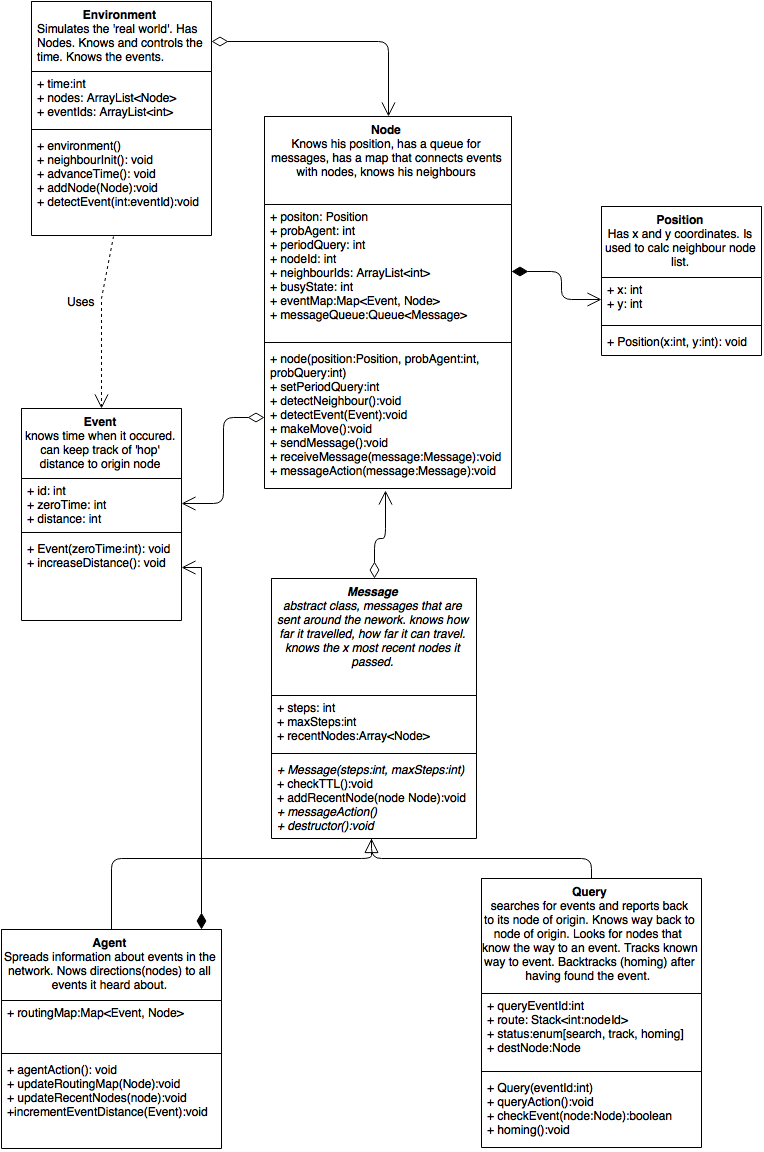
\includegraphics[width=\textwidth]{uml.png}
\caption{\textit{UML diagram for implementing a sensory network application
  that allows testing of the rumour routing algoritm.}}
\label{fig:uml}
\end{figure}



\section{Limitations and Future Development}

\section{Testing Framework}


\section{Reflections and Account for Individual Contributions}
\subsection{Johan Eklund}
We had a pretty good idea what we wanted to do right from the first
meeting. We made a solid UML diagram early on and we used it to make
pseudo-code that helped us a lot through the implementation of the
code.
We got a group chat and a git setup early in the project which has
helped a lot.
We had an early idea of making unit tests before implementing code, in
the end we did mostly the other way around, which made the tests a bit
redundant.
Differences in knowledge of the different tools has made some of the
group members spend a lot of time learning the tools and not
contribute as much as the more knowledgeable members. More meetings
and joint programming may have helped.
The problem specification can be read in different ways and a lot of
different solutions can be made for whatever you believe the
assignment to be. I assume this is part of the idea of the assignment.
I made the initial CRC suggestion that later became our first
UML-diagram. Worked on the position class and the main class that in
the final version became RumourRoutingApp. Made other small
contributions to other classes among them exceptions for a couple of
classes. Wrote JUnit tests working with Tommie. Worked on the final
report. Had some fierce battles with git.

\subsection{Tommie Lindberg}
\subsection{Jakob Lundin}
\subsection{Lorenz Gerber}

\addcontentsline{toc}{section}{\refname}
\bibliography{references}

\end{document}
